% !TeX root = ../Rules.tex
% !TeX spellcheck = en_US
\section{Field Technical Drawings}
\label{sec:technical_drawings}

\subsection{S-Field}

\centerline{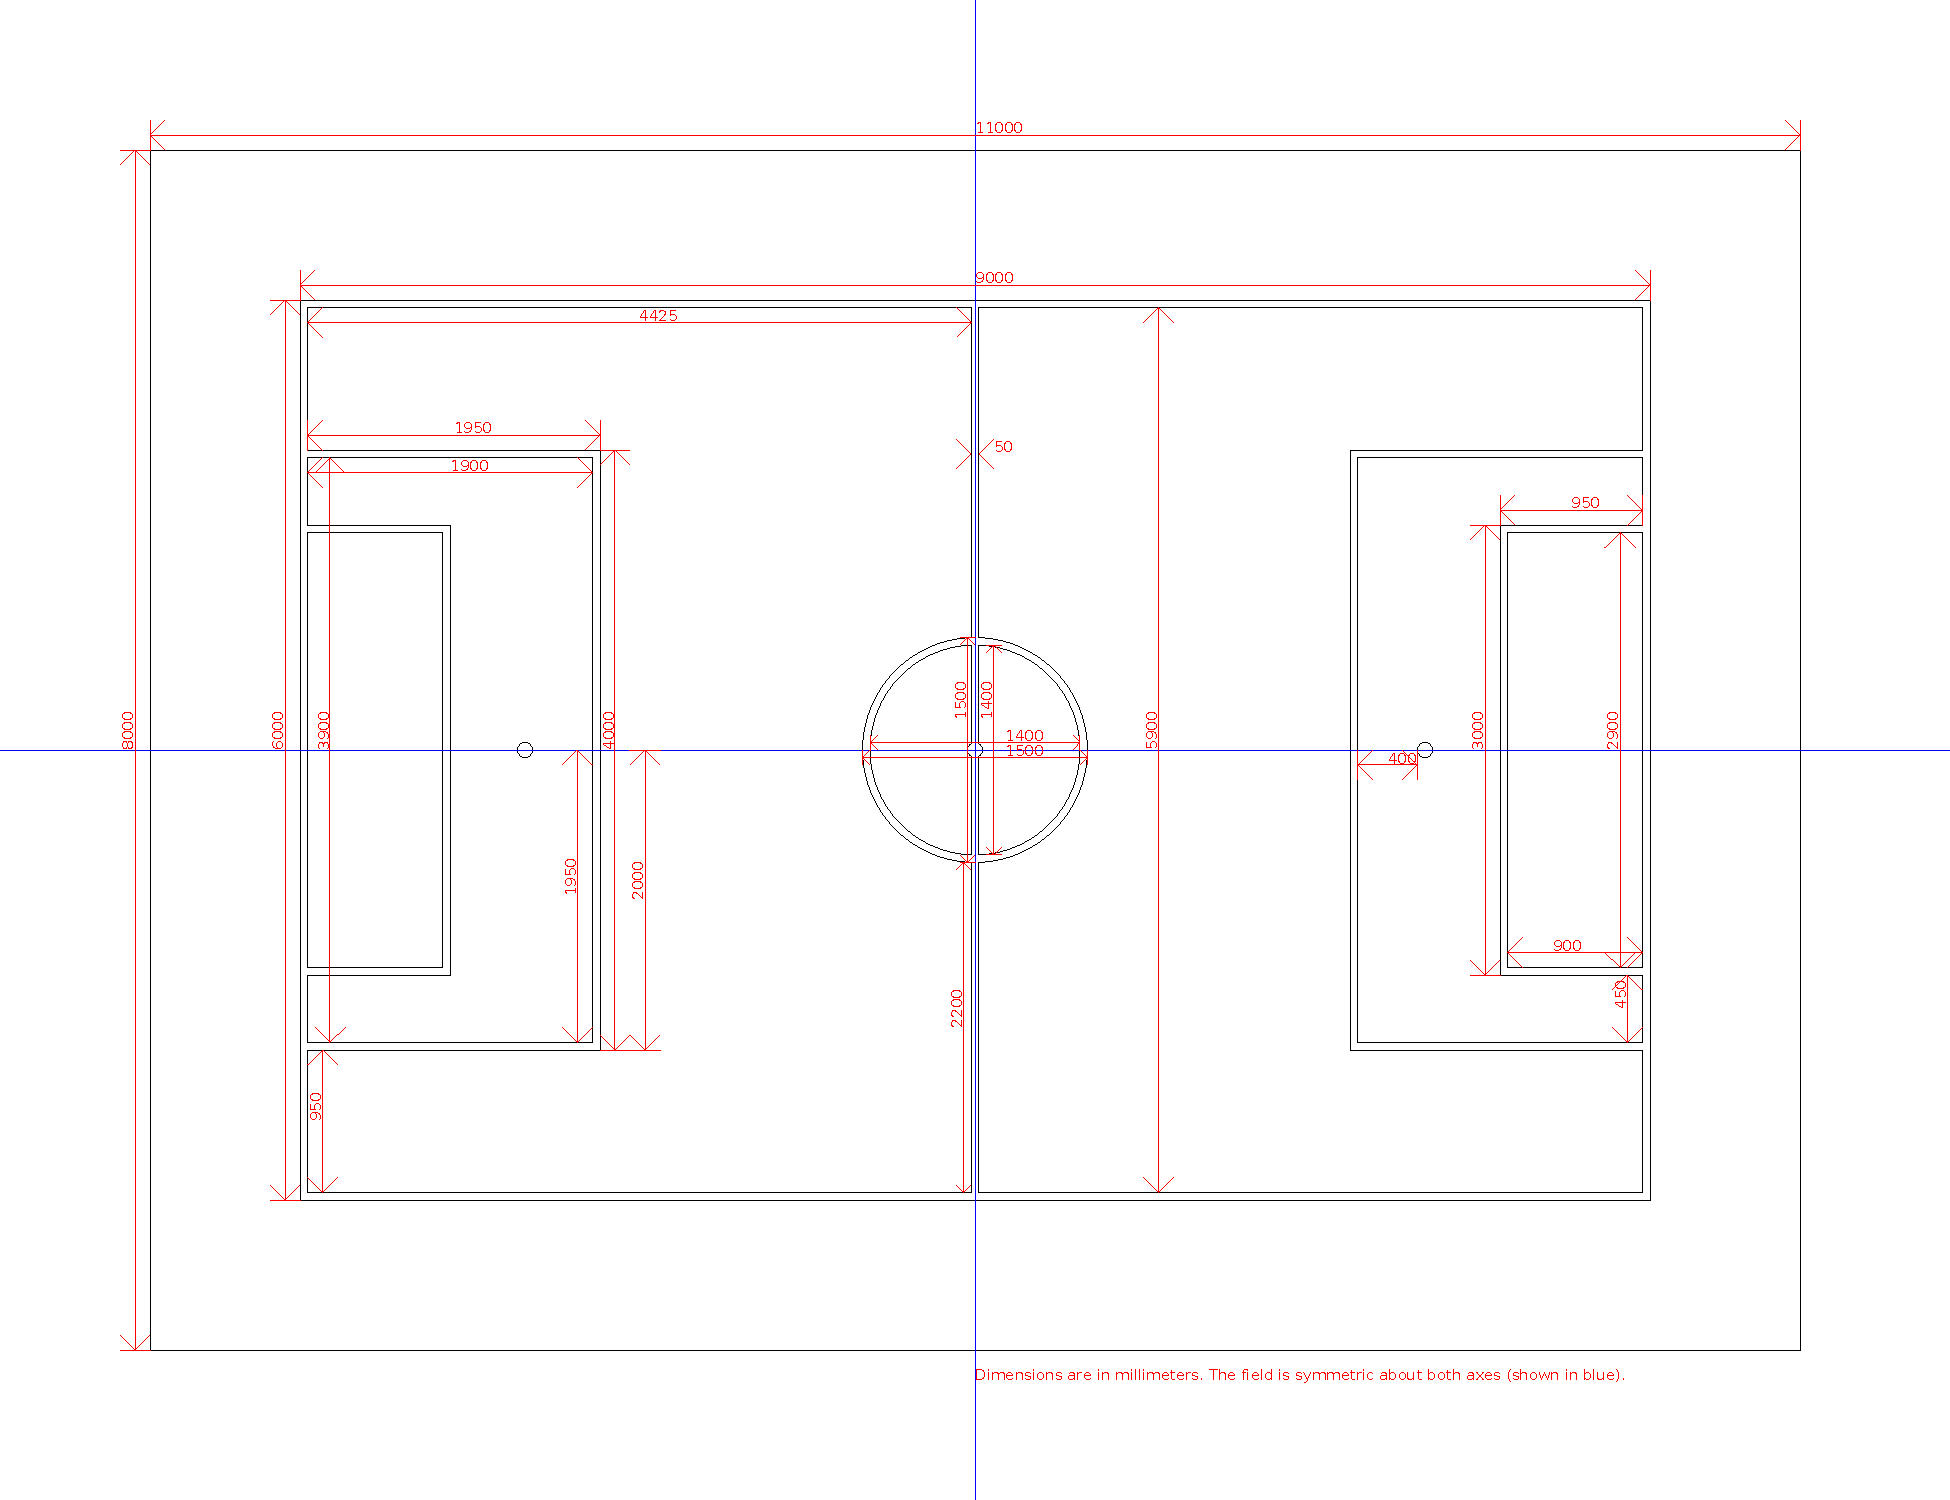
\includegraphics[angle=90,origin=c,width=0.95\columnwidth]{figs/field_hsl_s_2026_technical.pdf}}
\centerline{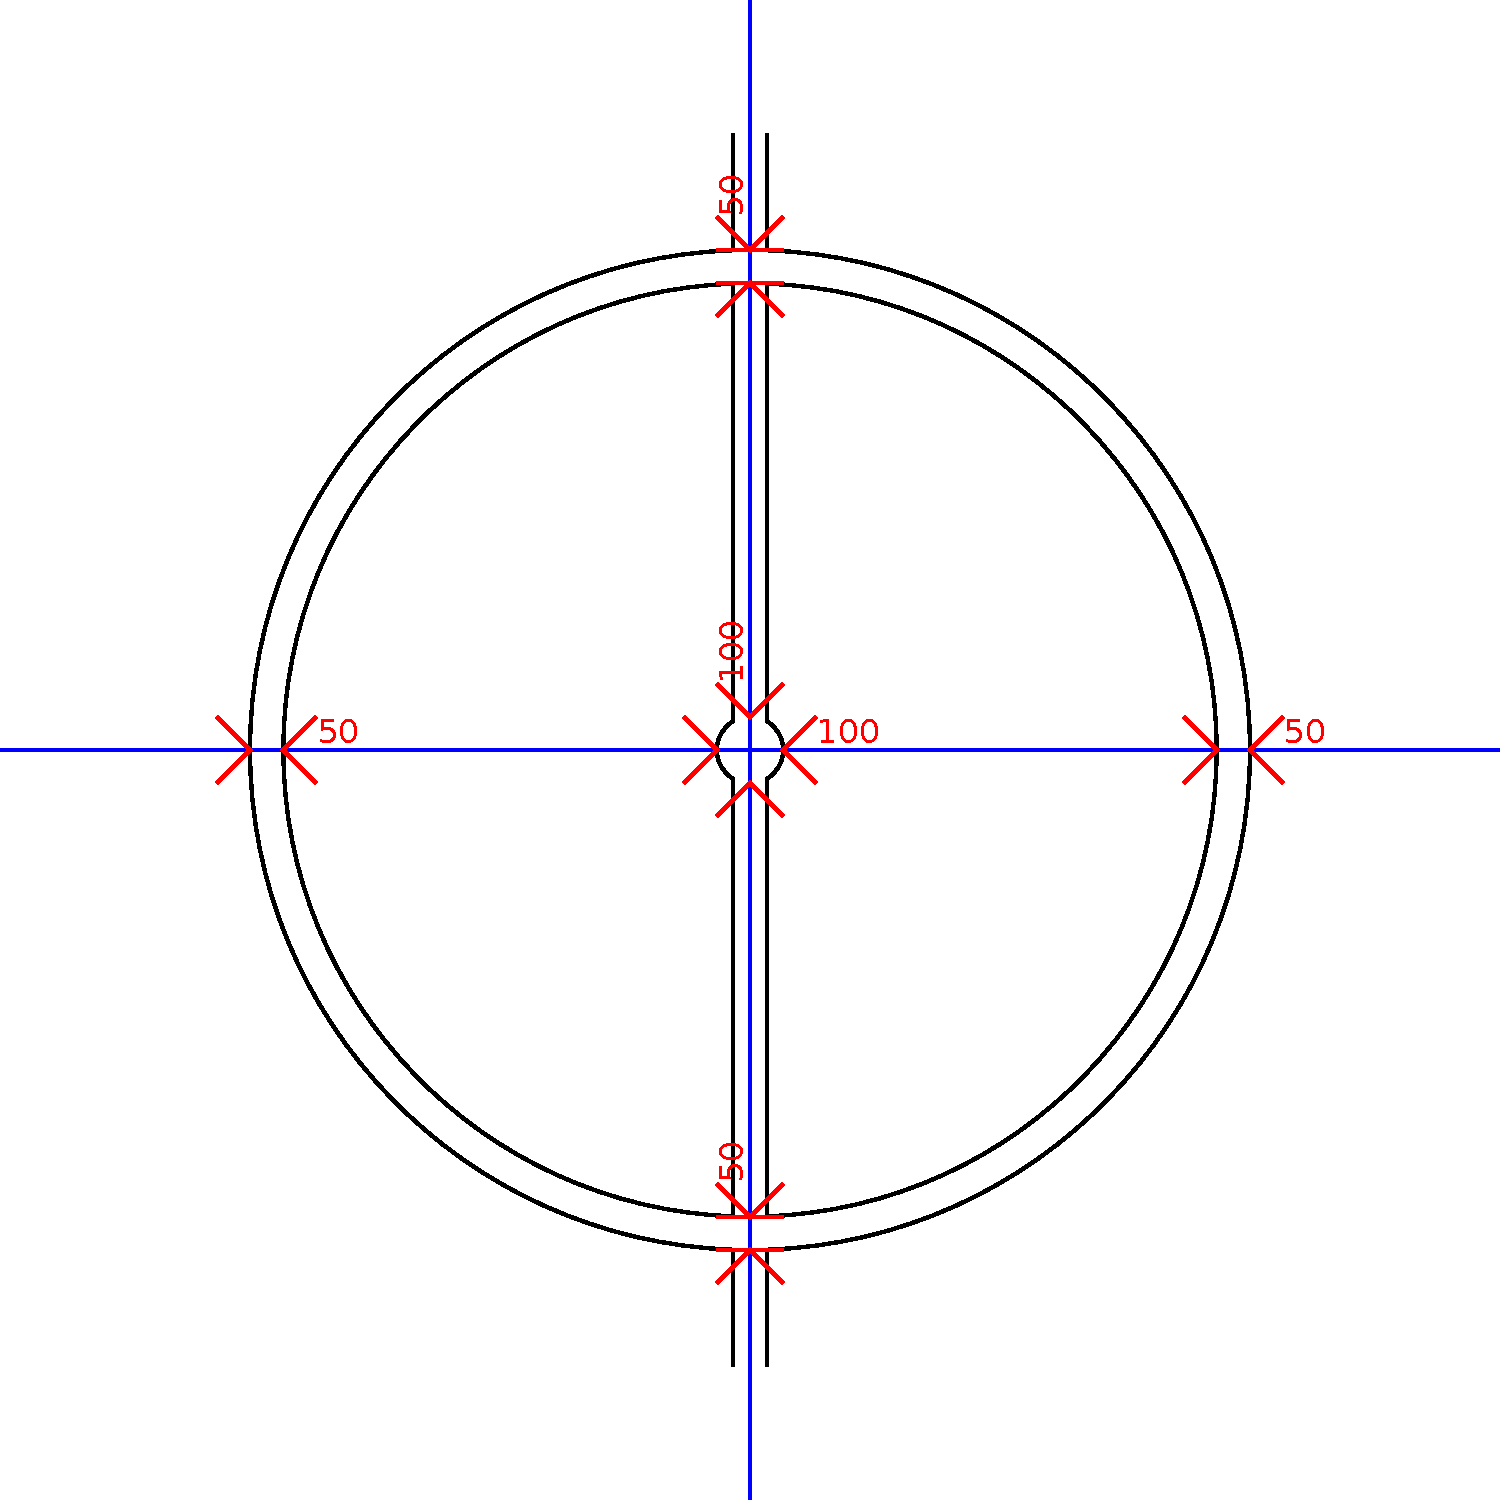
\includegraphics[angle=90,origin=c,width=0.5\columnwidth]{figs/field_hsl_s_2026_technical_cc.pdf}}
\centerline{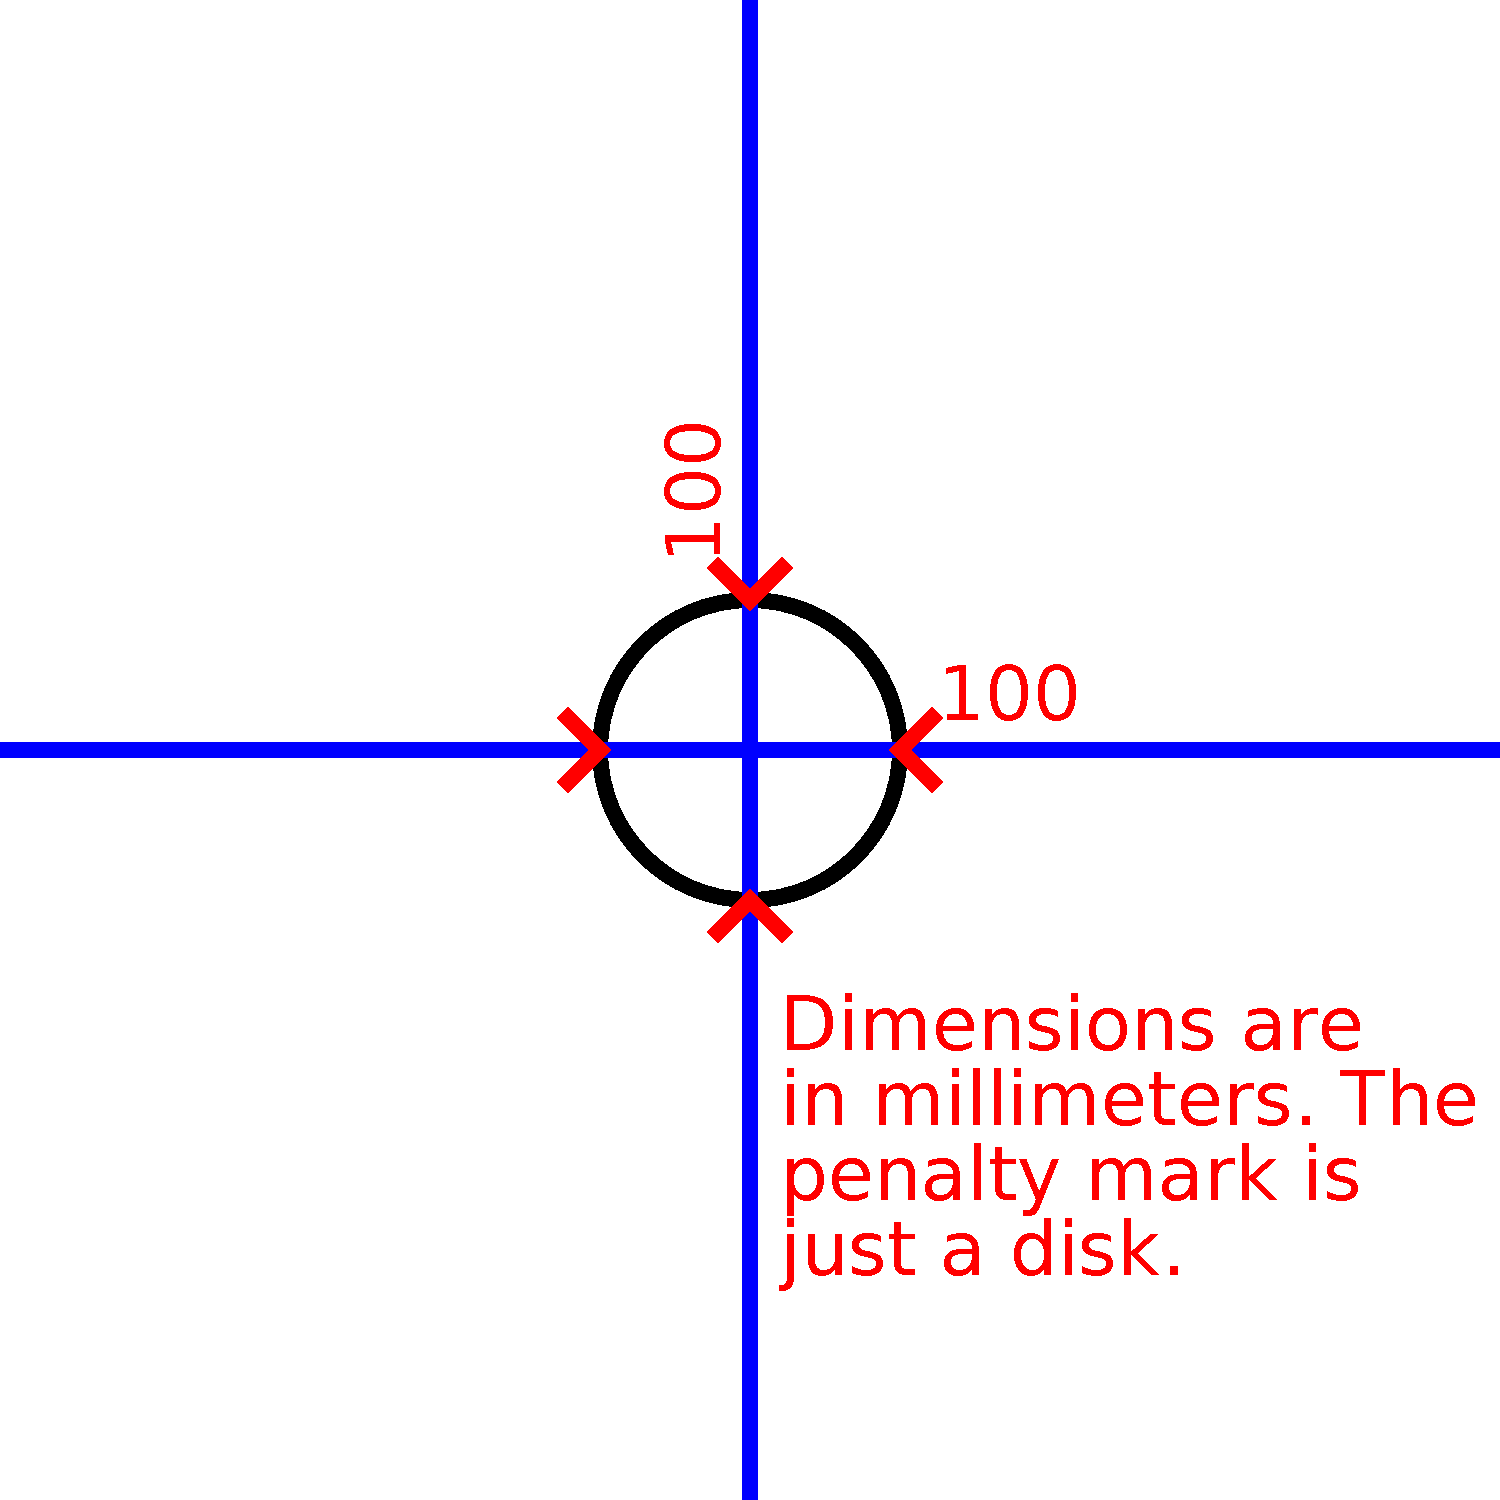
\includegraphics[origin=c,width=0.5\columnwidth]{figs/field_hsl_s_2026_technical_pm.pdf}}

\subsection{M-Field}

\centerline{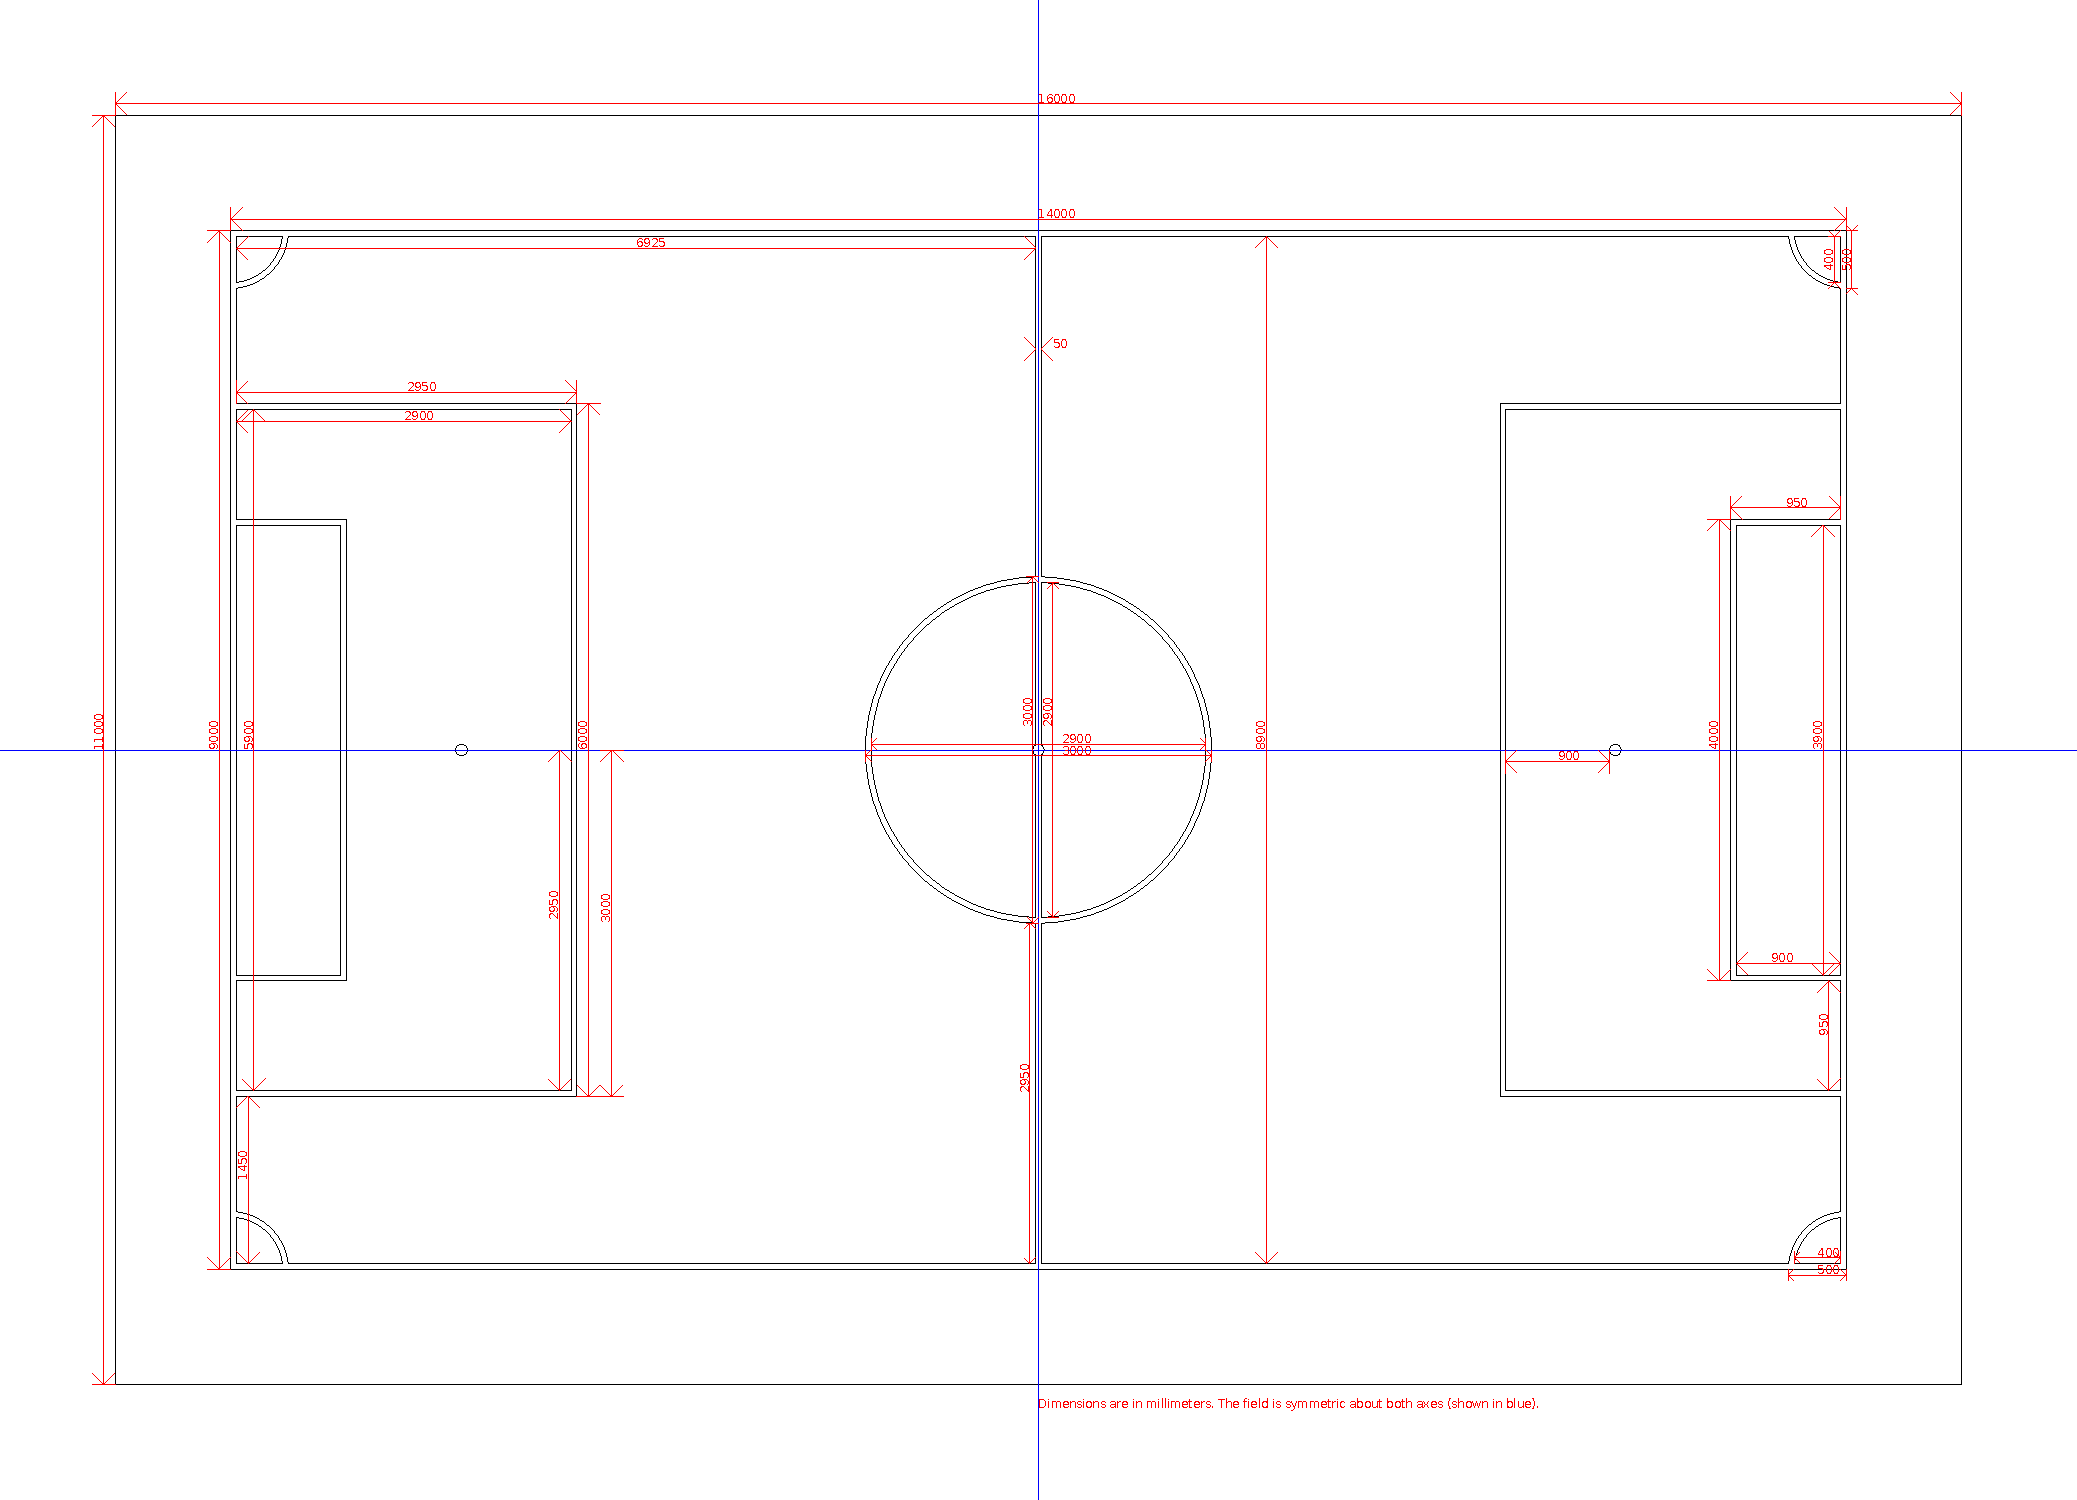
\includegraphics[angle=90,origin=c,width=0.95\columnwidth]{figs/field_hsl_m_2026_technical.pdf}}
\centerline{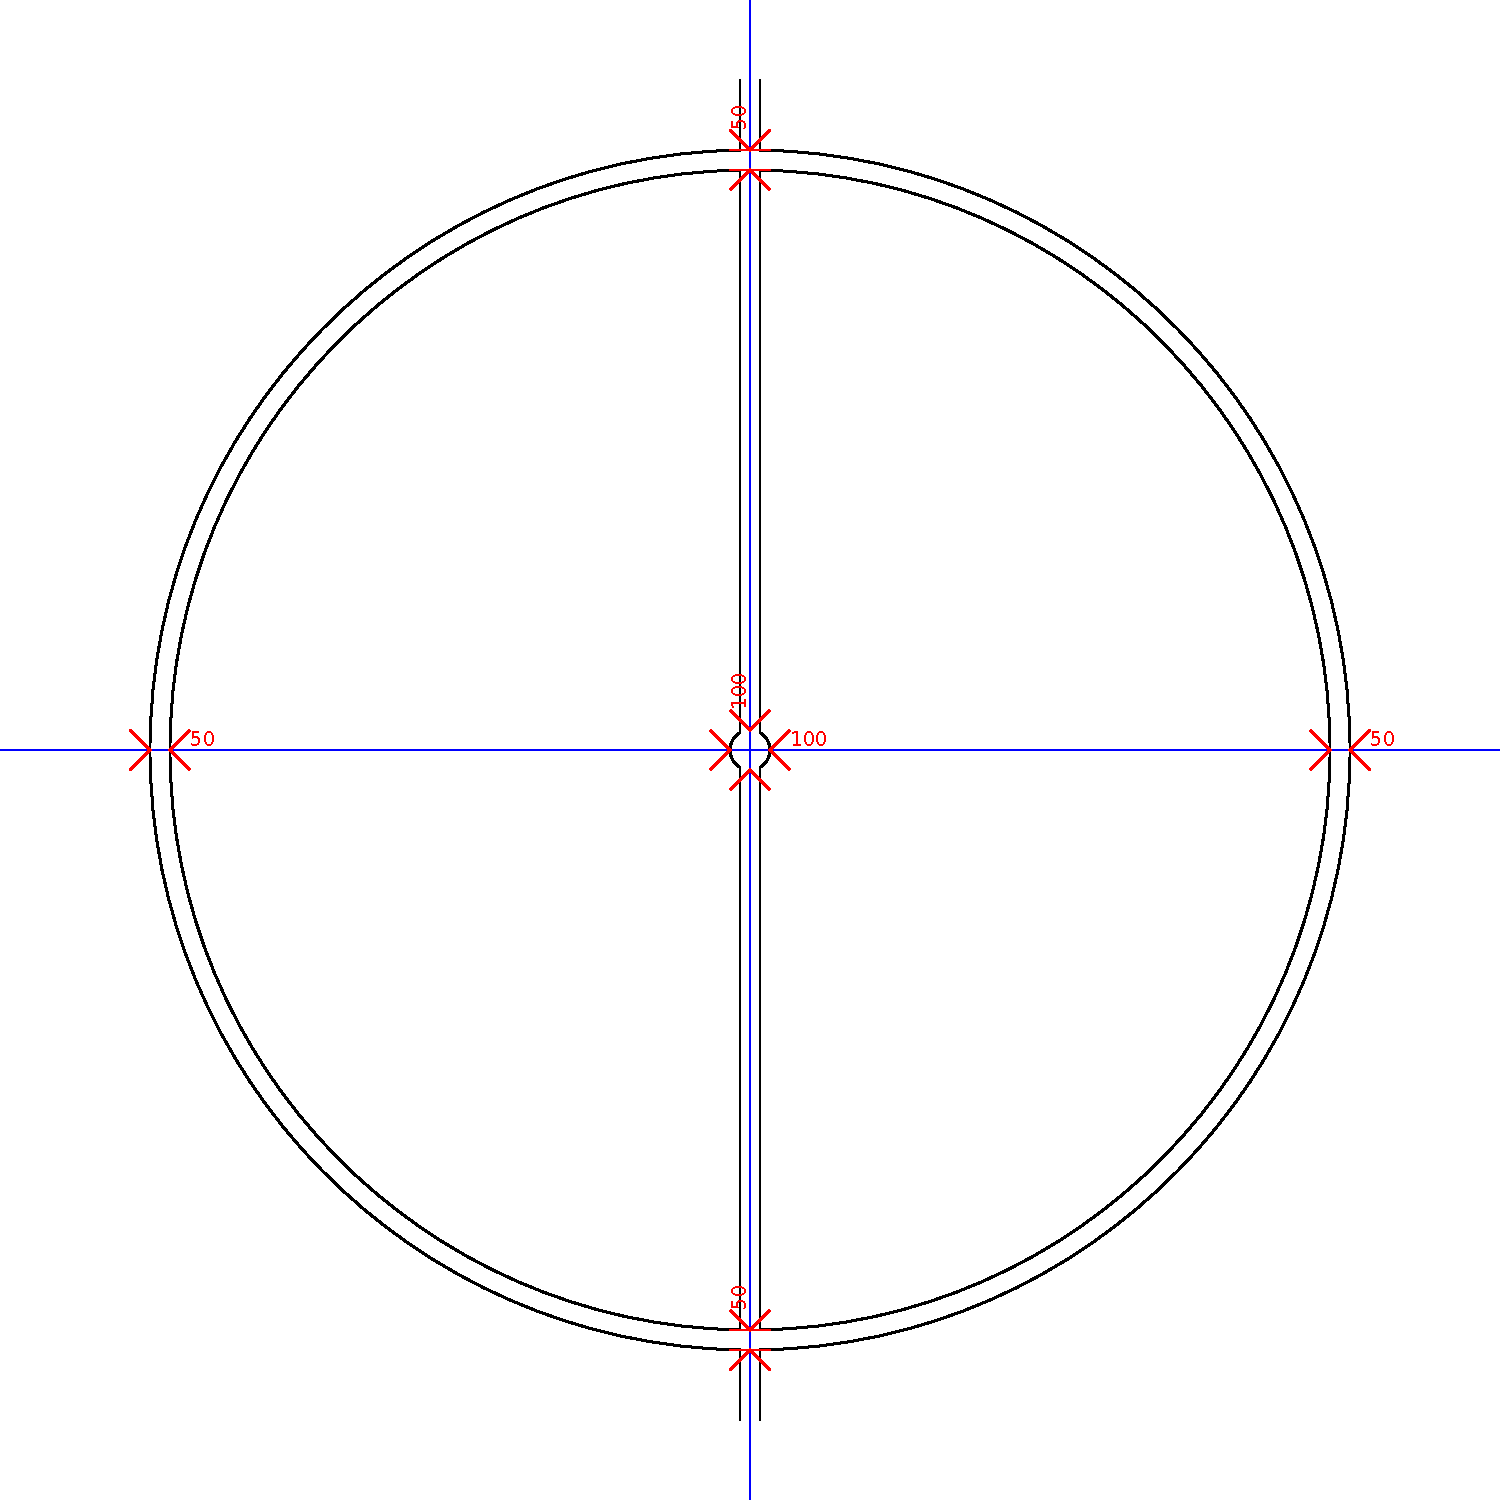
\includegraphics[angle=90,origin=c,width=0.5\columnwidth]{figs/field_hsl_m_2026_technical_cc.pdf}}
\centerline{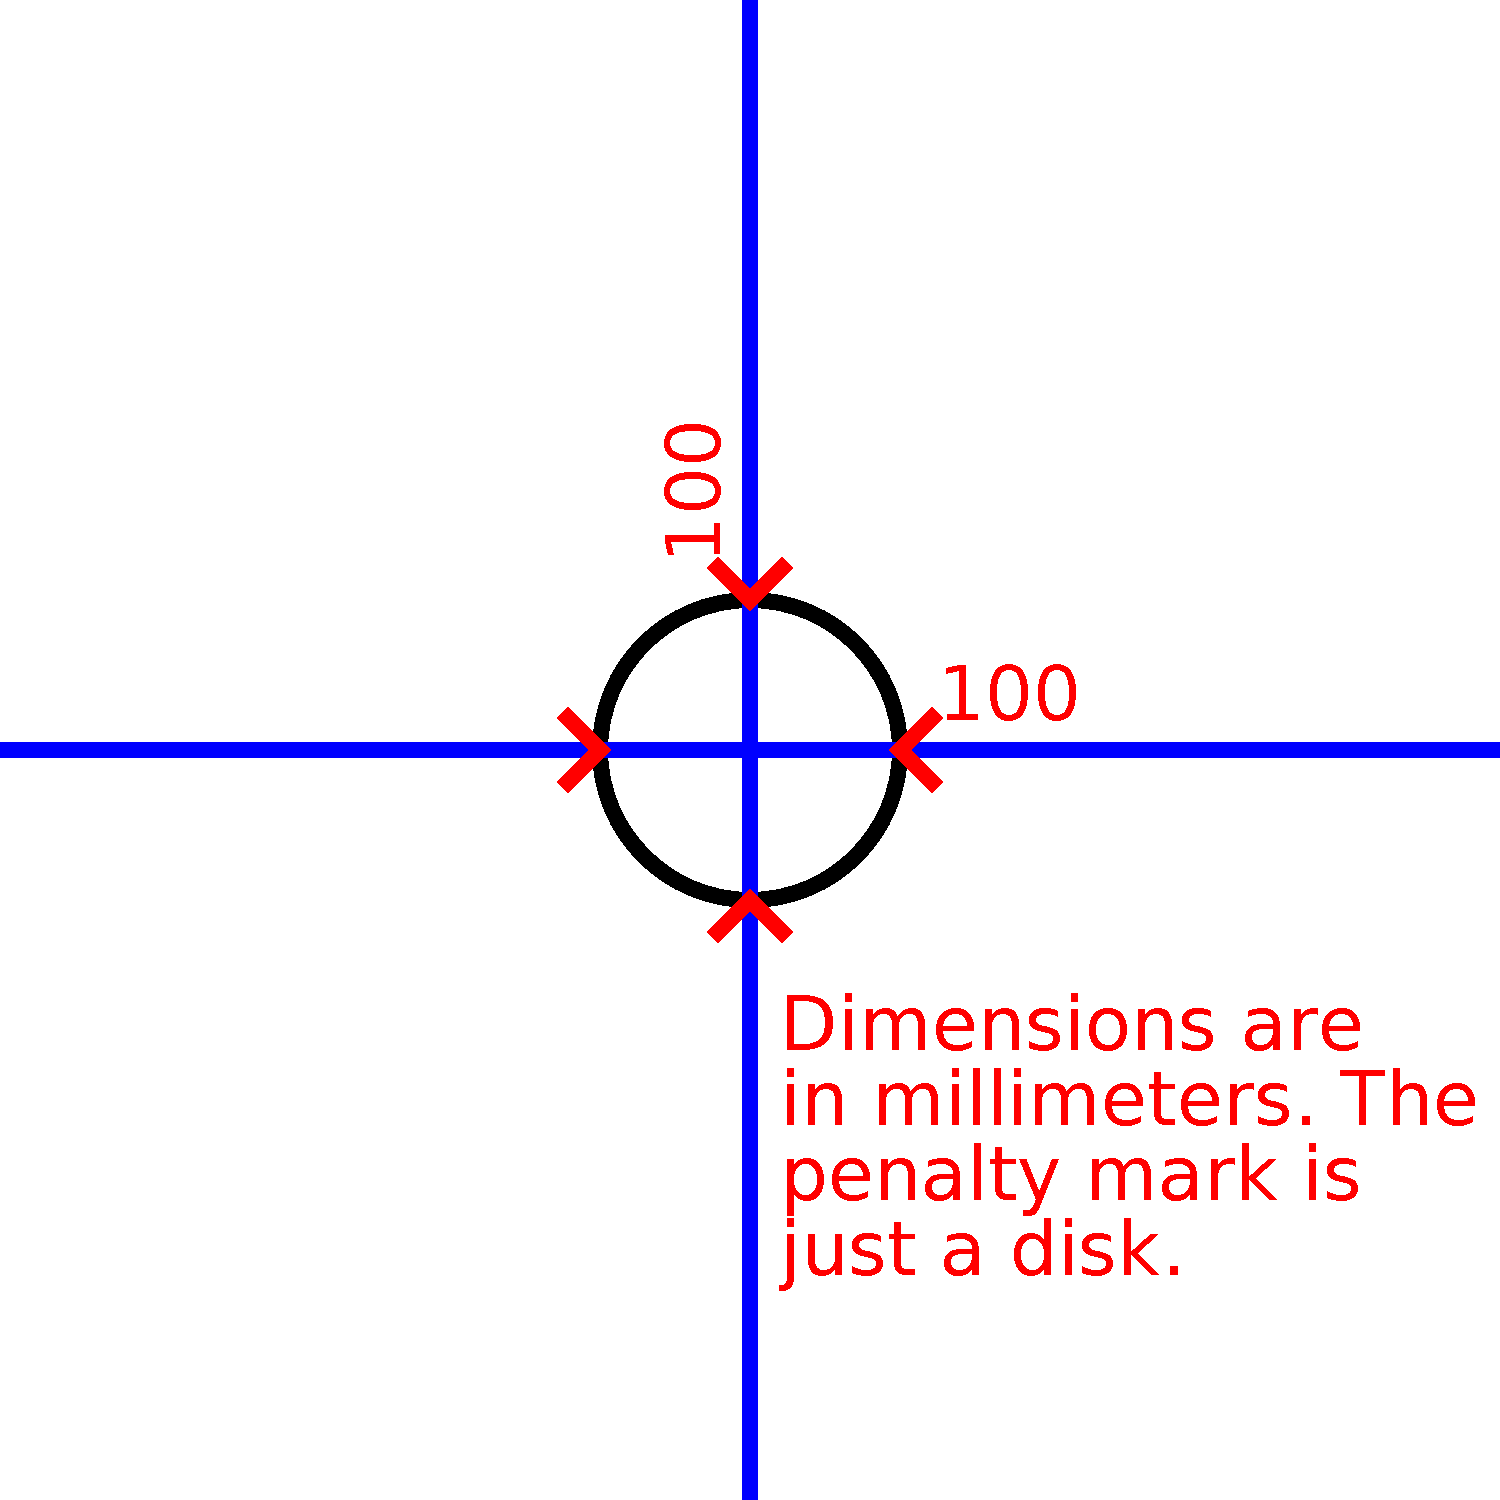
\includegraphics[origin=c,width=0.5\columnwidth]{figs/field_hsl_m_2026_technical_pm.pdf}}

\subsection{L-Field}

\centerline{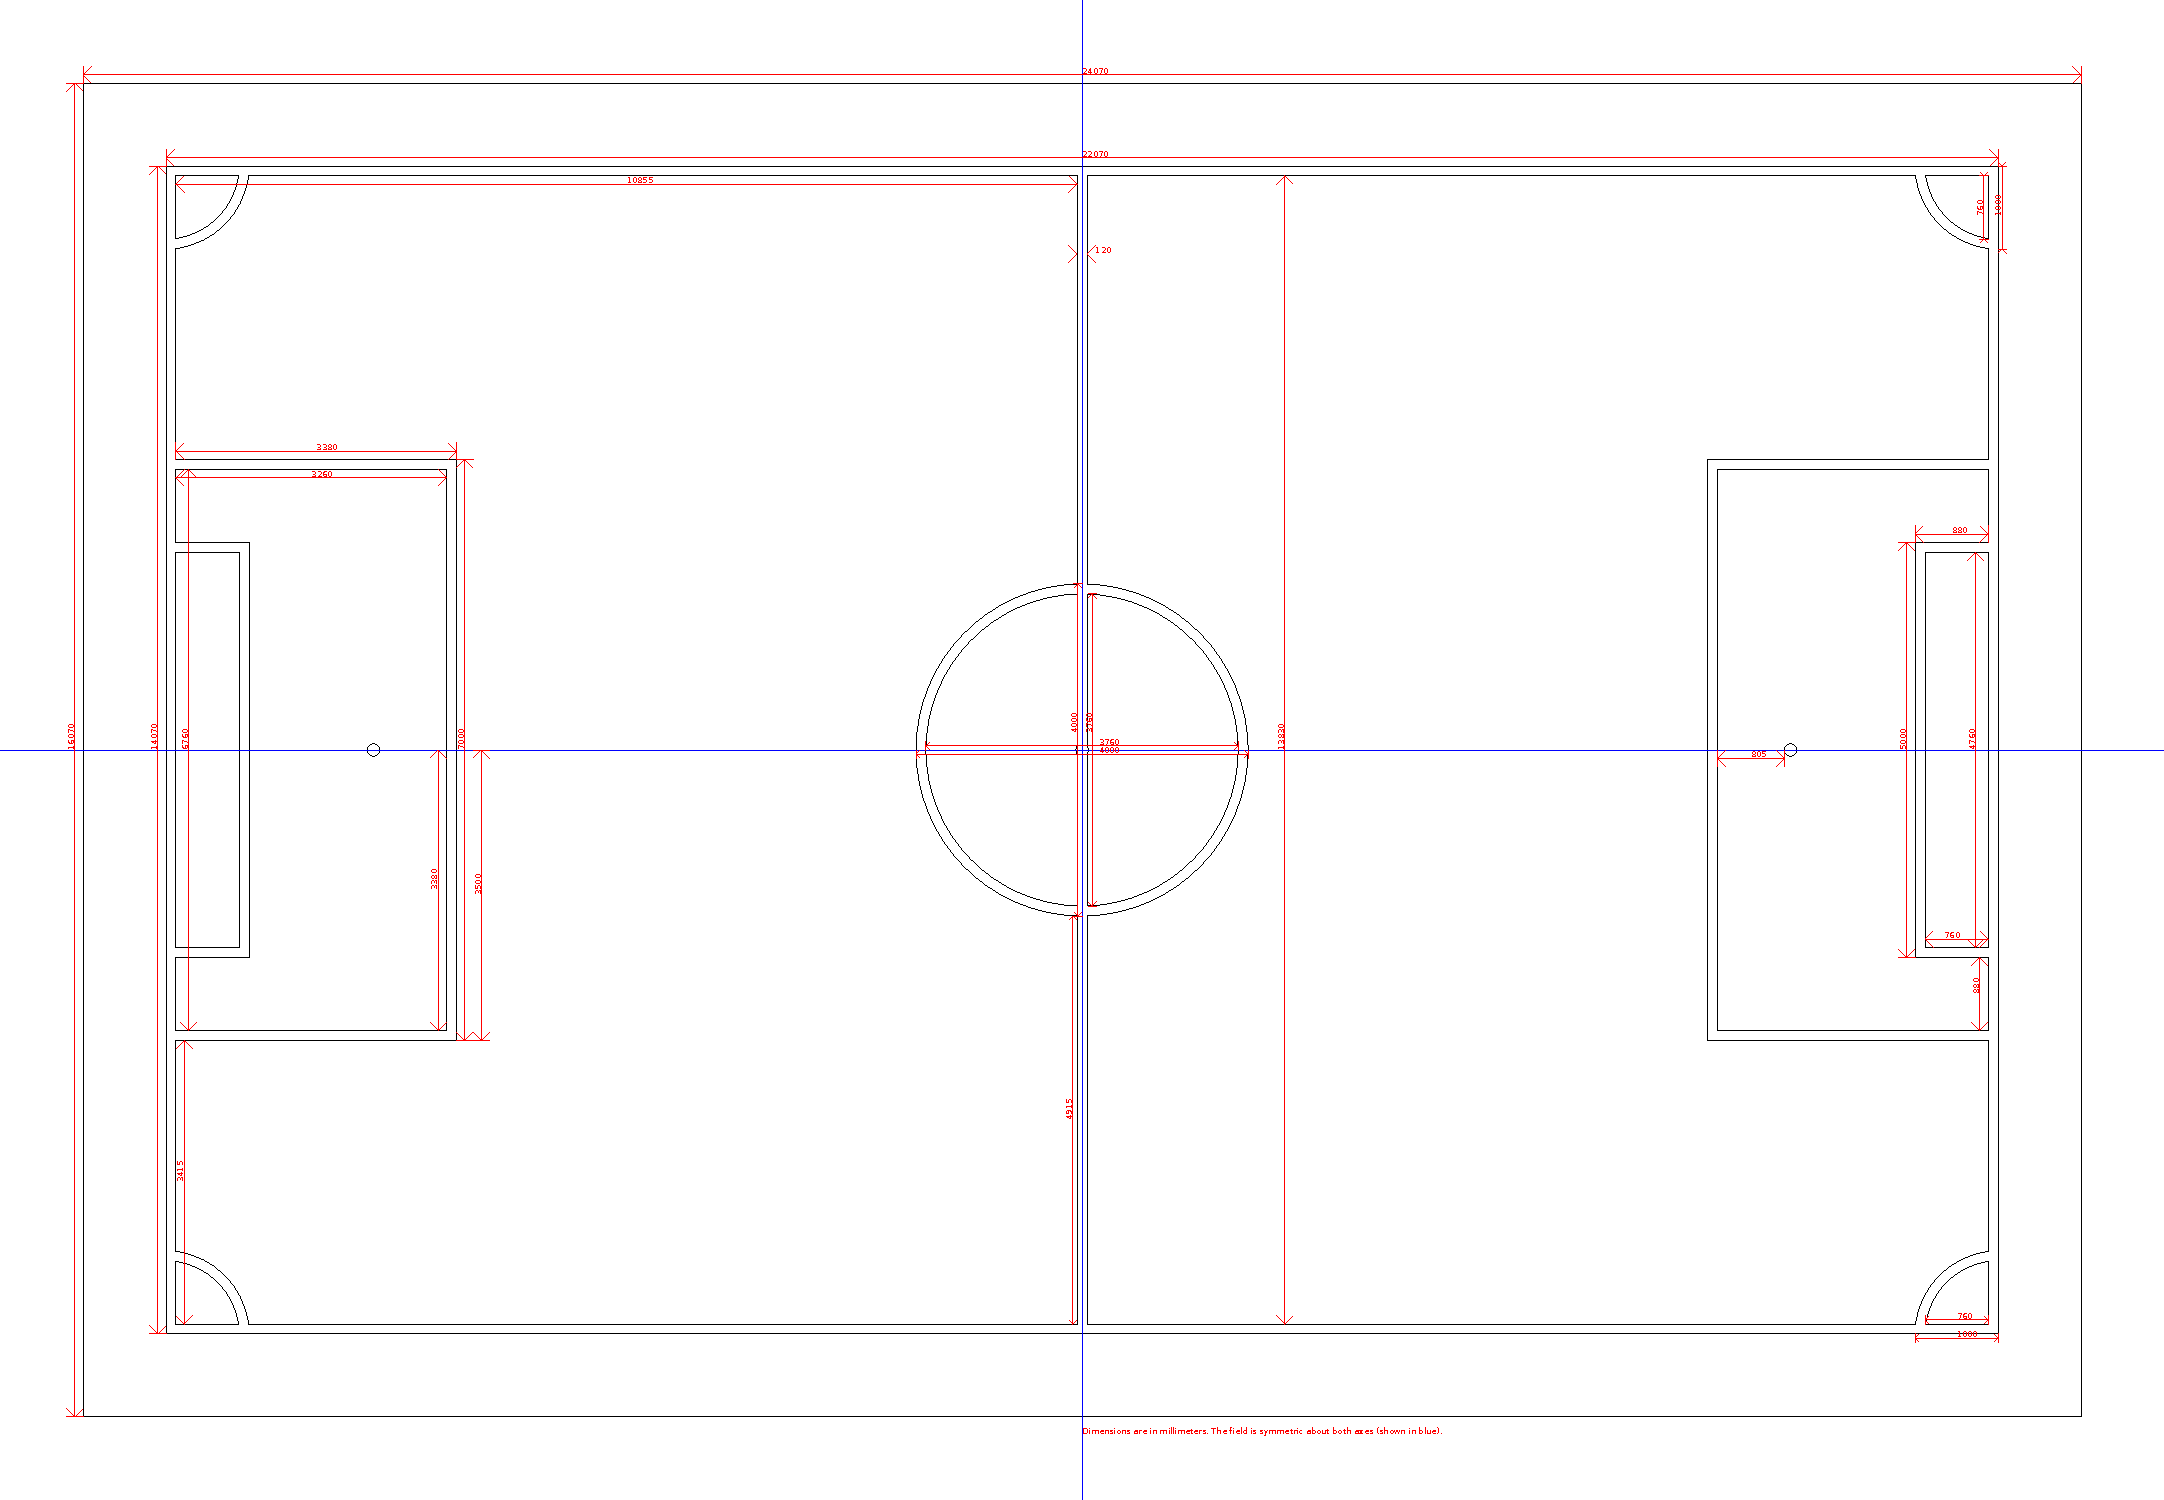
\includegraphics[angle=90,origin=c,width=0.95\columnwidth]{figs/field_hsl_l_2026_technical.pdf}}
\centerline{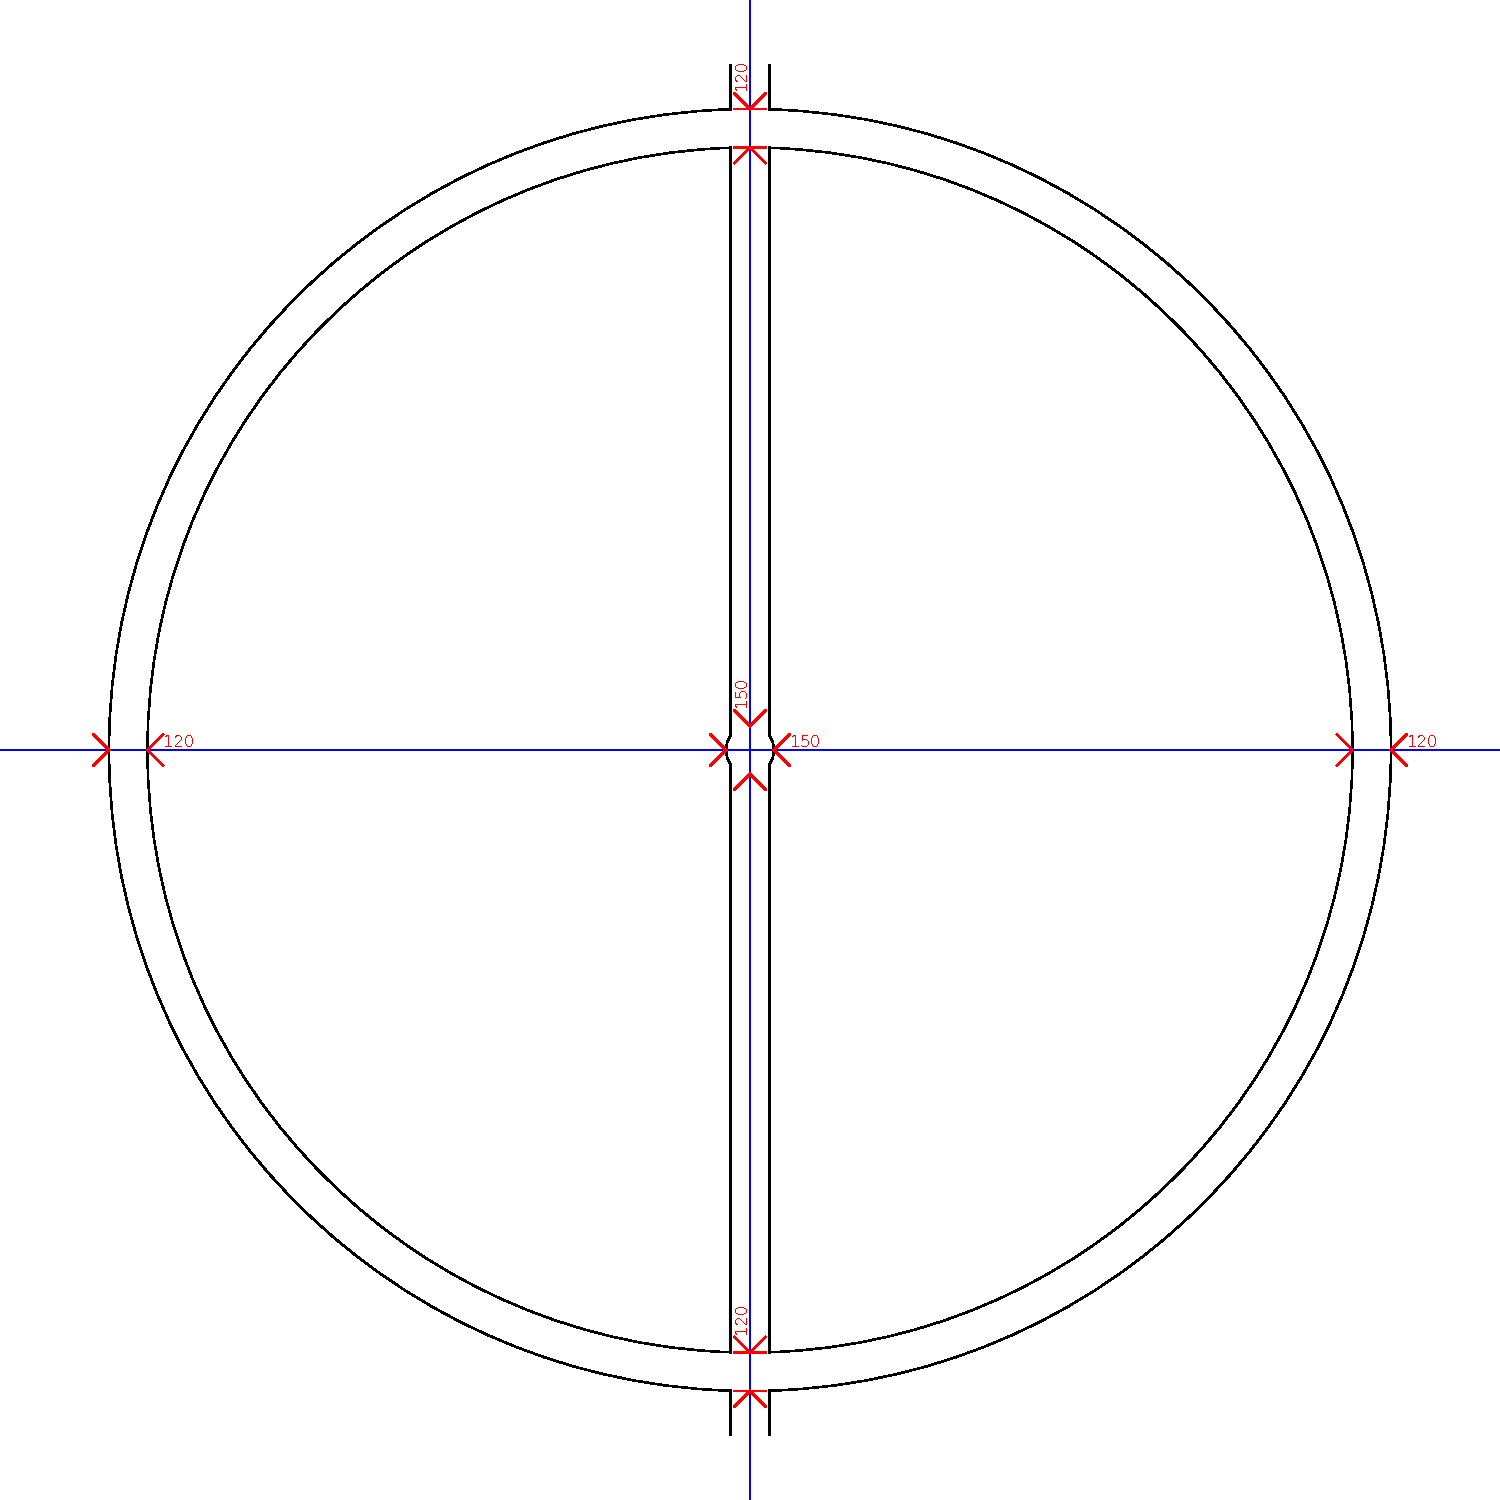
\includegraphics[angle=90,origin=c,width=0.5\columnwidth]{figs/field_hsl_l_2026_technical_cc.pdf}}
\centerline{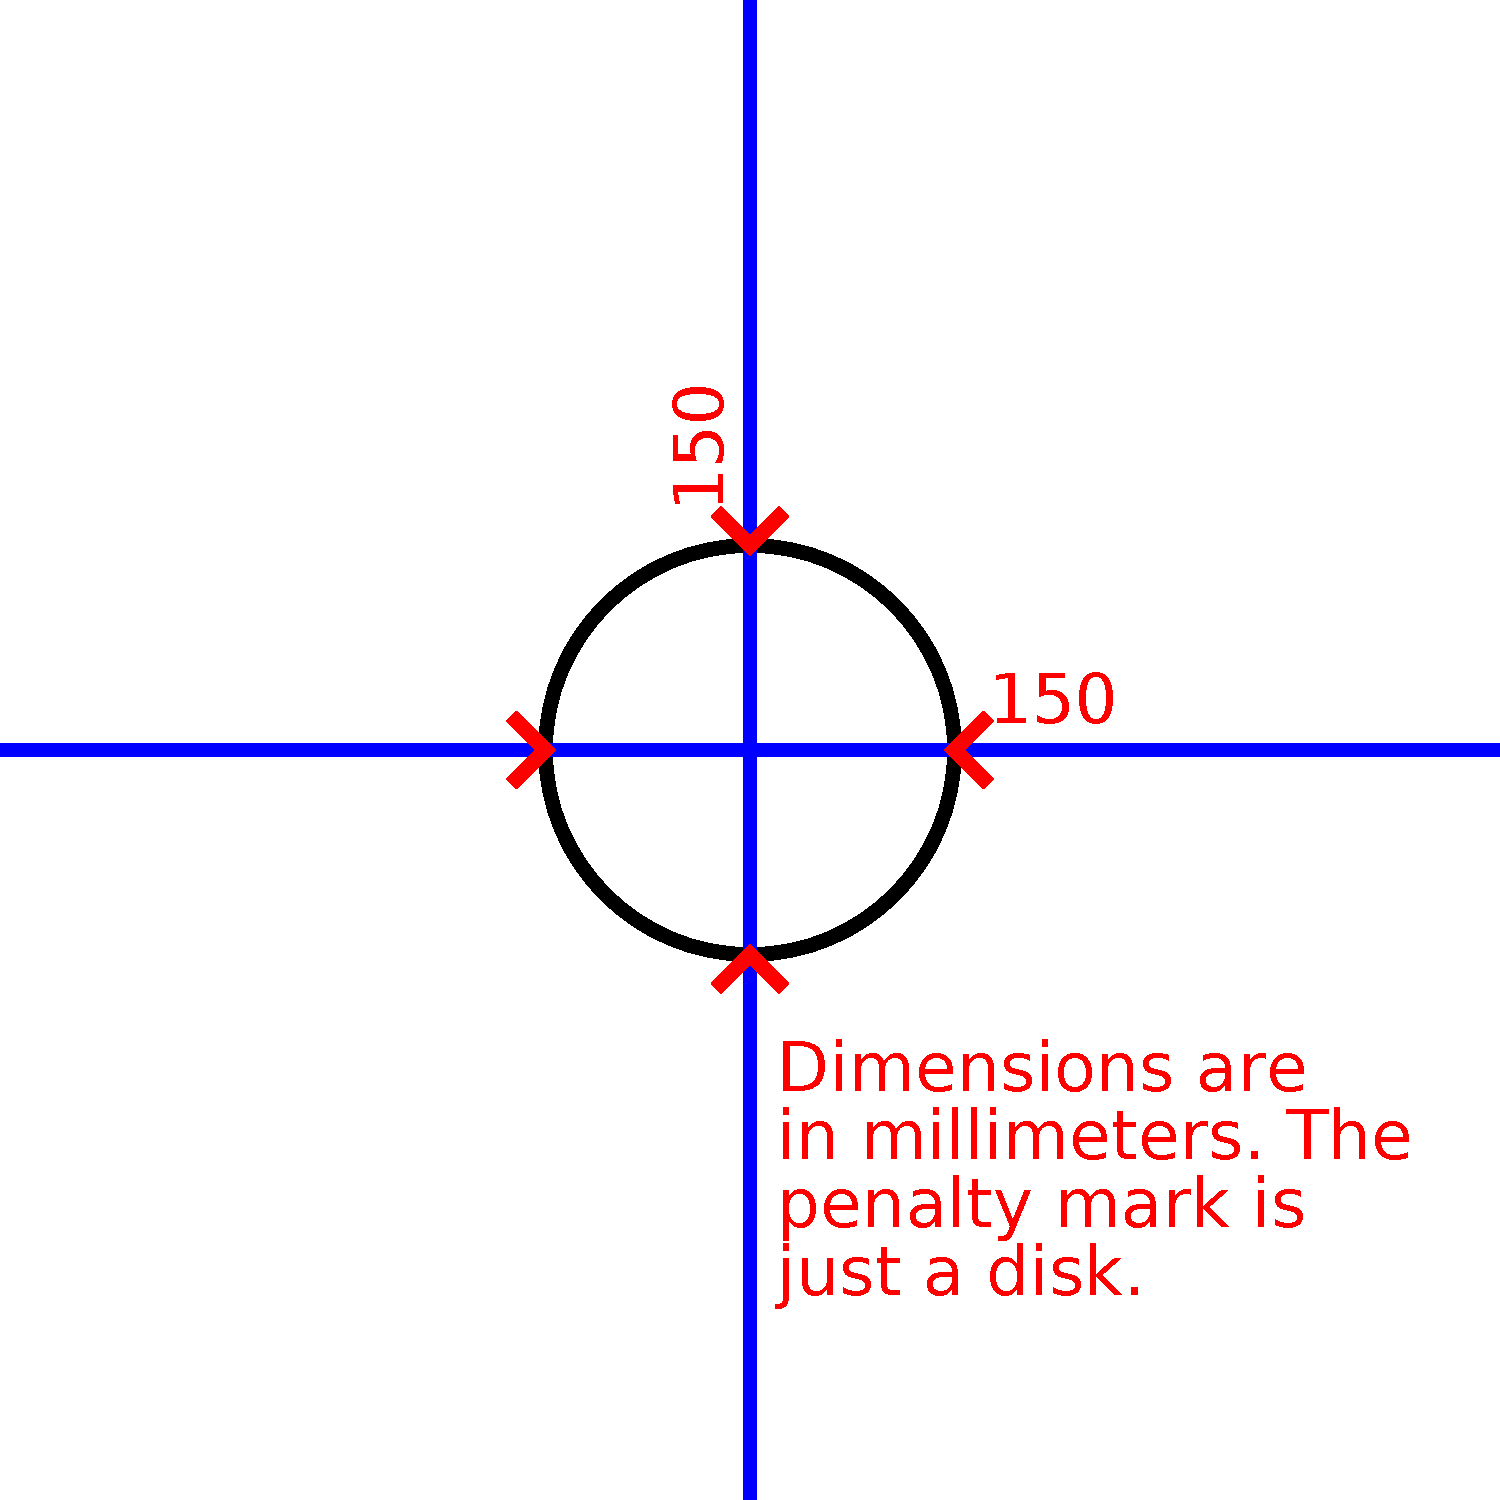
\includegraphics[origin=c,width=0.5\columnwidth]{figs/field_hsl_l_2026_technical_pm.pdf}}
